\documentclass[10pt, a4paper]{article}
\usepackage[utf8]{inputenc}
\usepackage{amsrefs}
\usepackage{tikz, wasysym}
\usetikzlibrary{automata,positioning}
\usepackage[]{algorithm2e}
\usepackage[]{csquotes}

\author{Sven Fiergolla}
\title{Research Methods \& wissenschaftliches Arbeiten mit \LaTeX}
\date{\today}

%TODOs: fix empfy last page
%		fill placeholher

\begin{document}
\maketitle

\paragraph{Abstract}
Dies ist eine Zusammenfassung über die Enstehung von Publikationen und wissenschaftlichen Arbeiten als solches, sowie den dabei notwendigen Einsatz von \LaTeX\  zur Ausarbeitung.
\par
\tableofcontents
\bigskip
\pagebreak %war nicht als 'illegaler' befehl klassifiziert
%\chapter{Wissenschaftliche Arbeiten}
\par

\section{Einführung}
\subsection{Gründe für die Publikaton}
\paragraph{}
Wissenschaftler haben verschiedene Beweggründe für die Veröffentlichung und den Verkauf an einen Verlag, ihrer Resultate aus Forschung, Kongressen o.ä.:
\par
\paragraph{}
\begin{itemize}
\item den Zeitpunkt einer Erkenntnis zu dokumentieren
\item die Ergebnisse der Arbeit zu teilen und sie zitierbar zu machen
\item sich im eigenen Fach einen Ruf zu verschaffen
\item Geld durch die Veröffentlichung zu erhalten \textit{(Tantieme)}
\item sich in der allgemeinen Öffentlichkeit bekannt zu machen
\end{itemize}
\par
\paragraph{}
Dazu verfassen sie sogenannte \enquote{Paper}, eine strukturierte Verschriftlichung der Resultate als wissenschaftliche Arbeit, zur Veröffentlichung.
Für uns, als Teilnehmer des \enquote{kleinen Studienprojekts}, ist die die Motivation, selbst Paper oder unsere Bachelor-Arbeit, in vergleichbarem Umfang und Struktur, zu verfassen.
\par

\subsection{Aufbau einer Arbeit}
\paragraph{}
Der grundsätzliche Aufbau einer wissenschaflichen Arbeit umfasst:
\begin{itemize}
\item den Titel, die Autoren und andere übergeordnete Informationen (Affiliation, Datum etc.)
\item ein Abstract (eine allgemeine Zusammenfassung)
\item eine Einführung mit den Grundlagen der Fragestellung
\item Ablauf der Forschung/Konferenz
\item technische Details/Beweis der Resultate
\item Conclusion (Fazit) und zukünftige Aspekte
\item References (Literaturverzeichnis)
\item Autor Contributions (Danksagung) und Conflict of Interests (Falls Interessenkonflikte bestehen, die Arbeit eine Auftragsarbeit war o.ä.)
\end{itemize}
\par

\section{Wissenschaftliche Arbeiten}
\subsection{Die \textit{DBLP}}
\paragraph{}
Das \enquote{Digital Bibliography \& Library Project}\textit{(DBLP)} ist eine bibliographische Sammlung von Publikationen und anderen Artikeln des Bereichs Informatik. Die Mehrheit der Einträge beschreibt Konferenz- und Juornalbeiträge. Insgesammt hostet die \textit{DBLP} über $3,3$ Mio. Artikel die alle frei online zugänglich sind.
\par 

\subsection{Fachzeitschriften}
\subsubsection{Allgemeines}
\paragraph{}
Grundsätzlich gilt es als großer Erfolg wenn eine Fachzeitschrift des einen Fachs das eigene Paper und damit die eigenen Forschungsergebnisse publiziert und damit einer deutlich gößeren Zielgruppe zugänglich macht. Es steigert den eigenen Ruf und die Reputation, auch die der Universität.\par

\subsubsection{Skandale/Risiken}
\paragraph{}
Zwischen 2003 und 2005 veröffentlichte der Verlag \enquote{Elsevier} ein Joural namens \enquote{Australasian Journal of Bone and Joint Medicine}. Dieses Journal vertrat gänzlich die Interessen des Konzerns \enquote{Merck}, welches ein führendes Technologieunternehmen im Bereich Healthcare ist.\par
\paragraph{}
Die Journale wirkten wie Fachzeitschriften und waren nicht als Auftragsarbeit gekennzeichnet. Soetwas birgt natürlich eine große Gefahr und zudem ist Missbrauch in anderen Magazinen nicht auszuschließen. Deshalb gewinnt Publikationen bei offenen Verlagen wie beispielsweise \enquote{Open Acces} immer mehr an Beliebtheit.\par
\paragraph{}
Zudem bestimmen einige wenige Medienhäuser die Preise der Lizenzen von wissenschaftlichen Arbeiten und Publikationen, die Verfasser des Papers treten häufig ihre Rechte an den Verlag ab. Dies ist ein weiterer großer Kritikpunkt am heutigen Publikationshergang. \par

\subsection{Der \textit{Ipact-Factor}}
\paragraph{}
Der \enquote{Impact Factor} \textit{(IF)} gibt die Höhe des Einflusses einer wissenschaftlichen Fachzeitschrift wieder, also den Ruf und das erreichte Publikum der Zeitschrift. Der Faktor gilt jedoch, als Qualitätsmaß einer Zeitschrift, als umstritten.\par

\subsection{Google Scholar}
\paragraph{}
Das zunehmend an Bedeutung gewinnende \textit{Google Scholar} dient als öffentliche Suchmaschine für wissenschaftliche Arbeiten und andere Veröffentlichungen. Zudem ist sichtbar, wie häufig ein Paper von anderen zitiert wurde.\par
\paragraph{}
\begin{center}

\includegraphics[scale=0.6]{GS1.png}
\end{center}\par
\paragraph{}
Zudem ist auf \textit{Google Scholar} auch sichtbar, wie häufig ein Forscher oder eine Arbeit von anderen Zitiert wurde, was einen gewissen Ruf wiederspiegelt.\par


\subsubsection{Der \enquote{h-index}}
\paragraph{}
Der \enquote{h-idex} oder auch \textit{Hirsch-Index}, gilt als Referenz für das Ansehen eines Wissenschaftlers in Fachkreisen. Dieser basiert auf den Zitationen der eigenen Veröffentlichungen des Wissenschaftlers. Ist eine große Anzahl von Publikaktionen eines Wissnschaflers häufig zitiert worden, so ergibt sich ein hoher h-index.\par
\paragraph{}
\begin{center}
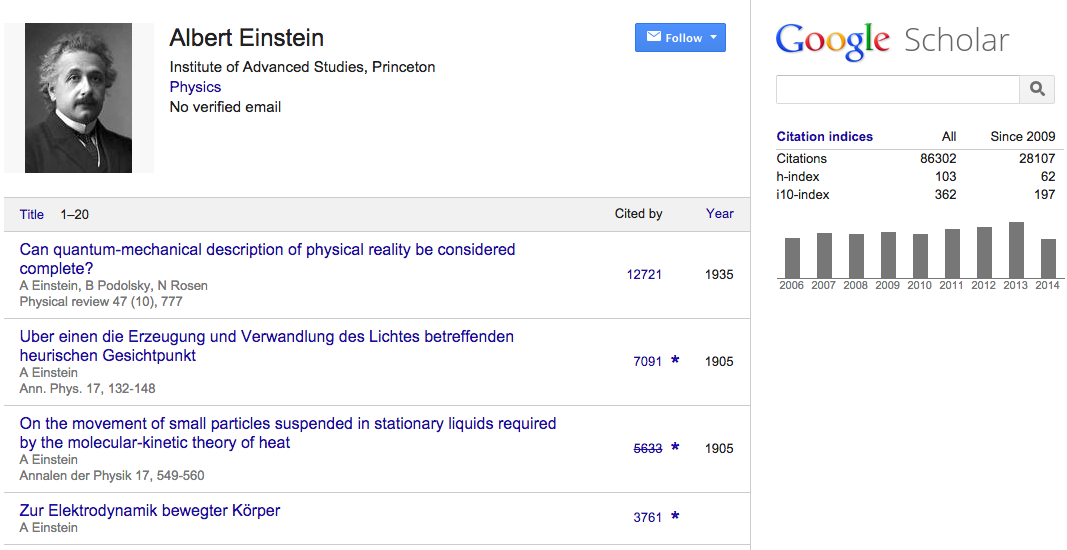
\includegraphics[scale=0.3]{ae.png}
\end{center}\par

\subsubsection{Der \enquote{i10-index}}
\paragraph{}
Der \enquote{i10-index} ist einfach die Anzahl der Publikationen eines Wissenschafters die mindestens 10 mal zitiert wurden. Diese Metrik wird zurzeit hauptsächlich bei \textit{Google Scholar} verwendet.

%\chapter{\LaTeX}
\section{Funktionalität von \LaTeX}
\subsection{Allgemeine Funktionalität}
Anders als in herkömmlichen Texteditoren wie \enquote{Word} oder \enquote{Open-Office}, welche nach dem \textit{WYSIWYG} (What you see is what you get) Prinzip arbeiten, muss der Autor seine zu formatierenden Passagen textuell auszeichnen. Es erfolgt also ein logisches Marup des Textes. Man nennt dieses Prinzip auch das \textit{WYSIWYAF}-Prinzip (What you see is what you asked for).\par
\subsection{Vorteile gegenüber \textit{WYSIWYG-Editoren}}
\paragraph{}
\LaTeX\ ist weitestgehen plattformunabhängig und eignet sich besonders für umfangreiche Arbeiten wie Dissertationen oder Bachelor/Master-Arbeiten, da \LaTeX\ ein sehr sauberes Layout generiert. Zudem bietet \LaTeX\ vielfältige Methoden für die Verschriftlichung von Formeln und weitere Features speziell für wissenschaftliche Arbeiten. Zudem lassen sich auch kleine Grafiken mit dem \enquote{Tikz}-Package erstellen.

\subsubsection{Graphen}
\paragraph{}
1.Graph


	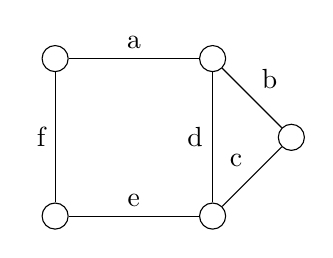
\begin{tikzpicture}[node distance=5cm,on grid,auto]
   
   \node[shape=circle,draw=black] (1) at (0,0) {};
   \node[shape=circle,draw=black] (2) at (0,2) {};
   \node[shape=circle,draw=black] (3) at (2,0) {};
   \node[shape=circle,draw=black] (4) at (2,2) {};
   \node[shape=circle,draw=black] (5) at (3,1) {};
   

    \path[-] (1) edge node {f} (2);
    \path[-] (2) edge node {a} (4);
    \path[-] (3) edge node {d} (4);
   	\path[-] (4) edge node {b} (5);
   	\path[-] (3) edge node {c} (5);
	\path[-] (1) edge node {e} (3);
	
	\end{tikzpicture}
\par
\paragraph{}
2.Graph
	

	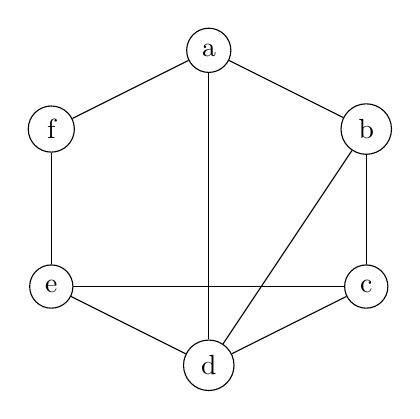
\begin{tikzpicture}[align=center, node distance=8cm,on grid]
   
   \node[shape=circle,draw=black] (1) at (0,0) {e};
   \node[shape=circle,draw=black] (2) at (0,2) {f};
   \node[shape=circle,draw=black] (3) at (4,0) {c};
   \node[shape=circle,draw=black] (4) at (4,2) {b};
   \node[shape=circle,draw=black] (5) at (2,3) {a};
   \node[shape=circle,draw=black] (6) at (2,-1) {d};
   

    \path[-] (1) edge node {} (2);
    \path[-] (2) edge node {} (5);
    \path[-] (3) edge node {} (4);
   	\path[-] (6) edge node {} (5);
   	\path[-] (4) edge node {} (5);
	\path[-] (1) edge node {} (3);
	\path[-] (1) edge node {} (6);
	\path[-] (3) edge node {} (6);
	\path[-] (4) edge node {} (6);
	
	\end{tikzpicture}
\par
\subsubsection{Pseudocode}
\paragraph{}
\begin{algorithm}[H]

 $q:=q_0$\\
 \For{$j:=1$ \KwTo $n$}{
 \While{$g[q,s_j]=$fail}{
  $q:=h[q]$\\}
  \If{q is in F}{\KwRet{\enquote{yes}}
 }}
  \KwRet{\enquote{no}}
 \par
 
 \bigskip
 
 \paragraph{}
 \caption{The Aho-Corasik algorithm for matching multiple keywords} \par
\end{algorithm}

\subsubsection{Tabelle}
\paragraph{}
\begin{tabular}{c||c c}
	\textbf{Bandinhalt} & \textbf{Übergangsfunktion} & \textbf{Gleichung}\\ \hline
	\\
	$...|\underbrace{B_{3,7,-,x}}|B_{13}|...$ &
	$\delta(B_{3,7,-,x},\alpha) = (B_{8,4,+,R},\beta,R)$ &  $(6)$\\ 
	\hline
	$...|B_{8,4,+,R}|\underbrace{B_{13}}|...$ & $\delta(B_{13},\beta) = (B_{13,1,-,L},\alpha,L)$ & $(2)$\\
	\hline
	$...|\underbrace{B_{8,4,+,R}}|B_{13,1,-,L}|...$ & $\delta(B_{8,4,+,R},\alpha) = (B_{8,3,+,R},\beta,R)$ & $(4)$\\
	\hline
	$...|B_{8,3,+,R}|\underbrace{B_{13,1,-,L}}|...$ &$\delta(B_{13,1,-,L},\beta) = (B_{13,2,-,L},\alpha,L)$  & $(3)$\\
	\hline
	$...|\underbrace{B_{8,3,+,R}}|B_{13,2,-,L}|...$ & $\delta(B_{8,3,+,R},\alpha) = (B_{8,2,+,R},\beta,R)$ & $(4)$\\
	\hline
	$...|B_{8,2,+,R}|\underbrace{B_{13,2,-,L}}|...$ & $\delta(B_{13,2,-,L},\beta) = (B_{13,3,-,L},\alpha,L)$ & $(3)$\\
	\hline
	$...|\underbrace{B_{8,2,+,R}}|B_{13,3,-,L}|...$ & $\delta(B_{8,2,+,R},\alpha) = (B_{8,1,+,R},\beta,R)$ & $(4)$\\
	\hline
	$...|B_{8,1,+,R}|\underbrace{B_{13,3,-,L}}|...$ & $\delta(B_{13,3,-,L},\beta) = (B_{13,4,-,L},\alpha,L)$ & $(3)$\\
	\hline
	$...|\underbrace{B_{8,1,+,R}}|B_{13,4,-,L}|...$ & $\delta(B_{8,1,+,R},\alpha) = (B_{8},\alpha,R)$ & $(5)$\\
	\hline
	$...|B_{8}|\underbrace{B_{13,4,-,L}}|B_{x}|...$ & $\dots$ & $(6)$\\
	\end{tabular}
	\par


%TODO:fix empty last page
\end{document}
